% !TeX encoding = UTF-8
\chapter[Nützliche Latex-Informationen]{Nützliche Latex-Informationen (Verwendung ist optional)}

\section{Latex-Distributionen und Editoren}

\LaTeX-Pakete und -Kompilierer haben den Vorteil, dass sie vollständig unabhängig von dem später verwendeten Latex-Editor installiert werden können. Sie werden in sogenannten Latex-Distributionen zusammengefasst. Empfehlenswerte Distributionen sind unter Windows MikTeX (\href{http://miktex.org/}{http://miktex.org/}) und unter OS~X MacTeX \href{https://tug.org/mactex/}{https://tug.org/mactex/}.

Die Auswahl des Latex-Editors erfolgt in der Regel nach individuellen Bedürfnissen und Geschmack.
Ein empfehlenswerter, plattformübergreifender Editor ist TeXstudio \href{http://texstudio.sourceforge.net/}{http://texstudio.sourceforge.net/}. Dieser bietet unter anderem die Möglichkeit, gewünschte Positionen der PDF-Vorschau unmittelbar im Quelltext anzuzeigen.
Ein weiterer verbreiteter Editor ist TeXnicCenter (\href{http://www.texniccenter.org/}{http://www.texniccenter.org/}).
Außerdem kann auch Visual Studio Code (\href{https://code.visualstudio.com/}{https://code.visualstudio.com/}) mit dem Latex-Plugin "`LaTeX Workshop"' (\href{https://marketplace.visualstudio.com/items?itemName=James-Yu.latex-workshop}{https://marketplace.visualstudio.com/items?itemName=James-Yu.latex-workshop}) verwendet werden. 
Dabei ist es möglich benutzerdefinierte \textit{Recipes} zu erstellen um verschiedene Befehle (z.B. Pdflatex, Latex, Bibtex, Biber, Makeindex, ...) nacheinander auszuführen.
Ein sinnvolles \textit{Recipe} für die Verwendung von Pdflatex ist beispielhaft \textit{pdflatex -> biber -> makeglossaries -> pdflatex*2} um zusätzlich zum Dokument auch das Literaturverzeichnis und die Nomenklatur zu erstellen.

Abschließend muss sich der Autor zwischen dem Latex- (PS/Dvi) und dem Pdflatex-Kompilierer entscheiden.
Die jeweilige Auswahl ist in den Einstellungen des verwendeten Editors zu treffen.\\

Pdflatex:
\begin{itemize}
	\item Fortschrittlicher als Latex
	\item Unterstützt folgende Bilddateitypen: PDF (Vektor), PNG, JPG.
	\item Unterstützt EPS-Bilder mit dem Paket "`epstopdf"' (bereits inkludiert).
	\item Nicht kompatibel mit alten Paketen, die nur mit PostScript-Dateien arbeiten.
\end{itemize}

Latex (PS/Dvi):
\begin{itemize}
	\item Funktioniert mit "`psfrag"' und anderen auf PS basierenden Paketen.
	\item Unterstützt ohne weitere Konvertierungen nur EPS-Bilder.
	\item Längere Kompilierungszeit
\end{itemize}


\section{Bild neben Tabelle}
Eine Tabelle neben einer Abbildung einfügen unter Berücksichtigung der zugehörigen Verzeichnisse (Tabellen, Abbildungen):
\begin{figure}[htbp]
%
	\begin{minipage}[t]{0.45\textwidth}
	\centering
	% \raisebox{2.5cm}{ %per hand
		\begin{tabular}{cc}
		\toprule
		Konfiguration & Parametersatz \\
		\midrule
		$1$ & $\{p_{1}, \: p_{2}, \: p_{5}\}$ \\
		$2$ & $\{p_{1}, \: p_{4}, \: p_{5}\}$ \\
		$3$ & $\{p_{2}, \: p_{3}, \: p_{4}\}$ \\
		\bottomrule
		\end{tabular}
	% }
	\captionof{table}{Definitionsbereich der Parameter zur Optimierung.} %ins tabellenverzeichnis einfügen
	\label{tab:bsp2}
	\end{minipage}
	\hfill
	\begin{minipage}[t]{0.45\textwidth}
		\centering
	  	\includegraphics[width=\textwidth]{images/logos/tud_logo_rgb}
  		\captionof{figure}{TU Dortmund Logo}
	\end{minipage}
\end{figure}


\section{Subcaption: Bild neben Bild und Tabelle neben Tabelle}

Das \textit{Subcaption} package (Beschriftung von Tabellen und Abbildungen mit a), b), ...) sollte ausschließlich gewählt werden,
wenn die zugehörigen Tabellen / Abbildungen auch wirklich kontextuell zusammengehören.

\begin{figure}[htbp]
        \centering
        \begin{subfigure}[b]{0.3\textwidth}
        		\centering
                \includegraphics[width=\textwidth]{images/logos/tud_logo_rgb} 
                \caption{TU Dortmund Logo}
                \label{fig:subfigure_tud_logo}
        \end{subfigure}%
        \quad %add desired spacing between images, e. g. ~, \quad, \qquad, \hfill etc.
          %(or a blank line to force the subfigure onto a new line)
        \begin{subfigure}[b]{0.3\textwidth}
        		\centering
                \includegraphics[width=0.3\textwidth]{images/logos/rst_logo_rgb} % relative width w.r.t. to the subfigure box
                \caption{RST Logo}
                \label{fig:subfigure_rst_rgb}
        \end{subfigure}
        \caption{Sammlung aller Logos}
        \label{fig:logos}
\end{figure}

Für lange Beschreibungstexte kann die \textit{Subfigure-Caption} leer gelassen werden. Eine Beschreibung mit Referenz zu den Buchstaben a),..., erfolgt dann in der allgemeinen Beschreibung.

Tabelle \ref{tab:parameter_tabellen} listet alle verwendeten Parameter auf. Tabelle \ref{tab:parameter_tabelle1} ...

\begin{table}[tb]
\caption{Hauptbeschriftung}
\centering
	\begin{subtable}[t]{.5\textwidth}
	\centering
			\caption{Tabelle links}
			\begin{tabular}{cc}
				\toprule
				Konfiguration & Parametersatz \\
				\midrule
				$1$ & $\{p_{1}, \: p_{2}, \: p_{5}\}$ \\
				$2$ & $\{p_{1}, \: p_{4}, \: p_{5}\}$ \\
				$3$ & $\{p_{2}, \: p_{3}, \: p_{4}\}$ \\
				\bottomrule
			\end{tabular}
			\label{tab:parameter_tabelle1}
	\end{subtable}%
	\begin{subtable}[t]{.5\textwidth}
			\centering
			\caption{Tabelle rechts}
			\begin{tabular}{cc}
				\toprule
				Konfiguration & Parametersatz \\
				\midrule
				$1$ & $\{p_{1}, \: p_{2}, \: p_{5}\}$ \\
				$2$ & $\{p_{1}, \: p_{4}, \: p_{5}\}$ \\
				$3$ & $\{p_{2}, \: p_{3}, \: p_{4}\}$ \\
				\bottomrule
			\end{tabular}
			\label{tab:parameter_tabelle2}
	\end{subtable}
	\label{tab:parameter_tabellen}
\end{table}




%
%
%
%%%%%%%%%%%%%%%%%%%%%%%%%%%%%%%%%%%%%%%%%%%%

\section{Zeichnungen und Matlab-Plots mit Tikz}
\label{sec:tikz}

Tikz ist ein umfangreiches \LaTeX-Paket, mit dem Bilder über Programmanweisungen erstellt werden können.
Zahlreiche Anleitungen und Beispiele können unter dem folgenden Link eingesehen werden:\\ 
\href{http://www.texample.net/tikz/examples/}{\emph{http://www.texample.net/tikz/examples/}}

Eine besonders nützliche Anwendung entsteht aus der Kombination mit dem Matlab-Plugin "`matlab2tikz"':\\
\href{http://www.mathworks.com/matlabcentral/fileexchange/22022-matlab2tikz}{\emph{http://www.mathworks.com/matlabcentral/fileexchange/22022-matlab2tikz}}\\
Hiermit können in Matlab erstellte Bilder in ein Tikz-Bild umgewandelt werden.
Ein Vorteil ist die einfache Möglichkeit, anschließend beliebige Attribute des Bildes beziehungsweise der Zeichnung anzupassen: Linienfarbe, -breite, -typ, Gitter, Legenden, Marker, u.a.

Die prinzipielle Vorgehensweise beginnt damit, den Tikz-Code zu erstellen:
\begin{enumerate}
	\item Matlab Zeichnung erstellen und in den Vordergrund holen (am Besten alle anderen Bilder schließen).
	Attribute der Zeichnung können auch schon hier angepasst werden (Gitter, Linienfarbe, -breite, Log-Skalierung,...).
	\item Nachdem "`matlab2tikz"' in den Matlab-Pfaden hinzugefügt wurde, kann das Bild konvertiert werden: \textit{matlab2tikz('myfile.tikz');}
	\item \textit{myfile.tikz} enthält nun den Tikz-Code der Abbildung.
\end{enumerate}

Tikz-Code kann innerhalb der \textit{tikzpicture}-Umgebung prinzipiell direkt im Latex Dokument verarbeitet werden.
Diese Variante skaliert jedoch nur schlecht mit den Kapazitäten des Latex Compilers.
Insbesondere bei mehreren Graphen aus Matlab, die mitunter viele Datenpunkte beinhalten können, kann der Compiler mit Speicherfehlern abstürzen.
Es ist daher ratsam, jedes Tikz-Bild als eigene Latex-Instanz zu kompilieren und dann als PDF einzubinden.
Um die Arbeit zu erleichtern gibt es hierfür das \textit{standalone}-Paket.
Den Tikz-Code in die \textit{standalone}-Umgebung einzubinden geht wie folgt:
\begin{enumerate}
	\item Die \textit{standalone}-Umgebung wird wie ein eigenständiges Latexdokument aufgebaut.
	Sie beginnt mit einer \textit{documentclass} und umschließt die \textit{tikzpicture}-Umgebung mit einer \textit{document}-Umgebung.
	In der Präambel werden entsprechende Pakete (z.B. Tikz, Pgfplots, Schriftarten, Mathematik, ...) geladen sowie benötigte Stile definiert.
	\item Wird als Klasse die \textit{standalone} Klasse gewählt, ist das resultierende PDF des eigenständigen Latexdokuments bereits auf die Maße des Inhalts/Bildes zugeschnitten.
	Ferner sollte die Klasse dieselbe Schriftgröße wie das spätere Hauptdokument haben.
	\item Das eigenständige Latexdokument kann entweder für sich kompiliert werden, oder per \textit{\textbackslash includestandalone[...]\{...\}}-Befehl in einem anderen (Haupt-)Dokument.
	Das Bild sollte bereits bei der Entstehung die richtigen Maße für das Zieldokument besitzen sodass die Option \textit{scale=1.0} gesetzt werden kann.
	Mit der Option \textit{mode=buildnew} wird das ausgelagerte Bild nur dann kompiliert, wenn es sich verändert hat.
	Damit lässt sich der Kompiliervorgang des Hauptdokuments im Falle von vielen Bildern erheblich beschleunigen.
	\item Die in einzelnen Instanzen erzeugten PDFs der ausgelagerten Bilder befinden sich im gleichen Ordner wie der Tikz-Code und können von dort auch schnell und einfach für andere Zwecke (Präsentation, ...) verwendet werden.
\end{enumerate}
Siehe als Beispiel einer eigenständigen Bildumgebung den Quelltext der Abbildung \ref{fig:tikz:x_square}.

Diese Vorlage ist so aufgebaut, dass sowohl die Pakete aus der Datei \textit{shared\_packages.tex} als auch die Befehle aus der Datei \textit{commands.tex} per \textit{\textbackslash input} in die \textit{standalone}-Umgebung eingebunden werden können.
In \textit{shared\_packages.tex} werden direkt auch die Dateien \textit{colordef.tex} und \textit{tikzdef.tex} eingebunden für eigene Farben und Tikzstile. 
Auf diese Weise müssen Pakete, Befehle, Farben und Stile nicht in jede \textit{standalone}-Umgebung kopiert werden, sondern können zentral angepasst werden.

\begin{figure}[h]
	\centering
	\includestandalone[mode=buildnew,scale=1.0]{images/tikz/Figure_X_Square}
	\caption{Quadratische Funktion}
	\label{fig:tikz:x_square}
\end{figure}


\subsection{Tikz-Plots anpassen}

Falls \texttt{matlab2tikz} verwendet wird, verwendet die Tikz-Umgebung zunächst die wissenschaftliche Darstellung von Zahlen, d.h. abhängig von Zehnerpotenzen.
Ist dies nicht gewünscht, können in die \textit{axis}-Umgebung die folgenden Befehle, oder eine Auswahl davon, eingefügt werden:

\begin{itemize}
         \item \texttt{scaled y ticks = false,} 
         \item \texttt{scaled x ticks = false,}
         \item \texttt{y tick label style={/pgf/number format/.cd, fixed, int detect, fixed zerofill, precision=3},}
         \item \texttt{x tick label style={/pgf/number format/.cd, fixed, int detect, fixed zerofill, precision=3}}
\end{itemize}

Die ersten zwei Befehle erlauben die Zusammenfassung der Zehnerpotenzen, sodass eine gemeinsame Zehnerpotenz an die Achse geschrieben wird.
Die unteren beiden Befehle stellen die notwendige Präzision ein.


\subsection{Zeichnen mit Tikz}

Tikz kann auch für Blockschaltbilder u.a. verwendet werden (siehe oben verlinkte Sammlung an Beispielen).
Anleitungen findet man bei Google wie Sand am Meer.

\begin{figure}[htb]
	\centering
	\begin{tikzpicture}[->,>=stealth',shorten >=1pt,auto,node distance=3cm, thick]
	 		\tikzstyle{main node}=[circle,fill=black!40,draw,font=\sffamily\Large\bfseries]
	 		\node[main node] (1) {1};
	 		\node[main node] (2) [below left of=1] {2};
	 		\node[main node] (3) [below right of=2] {3};
	 		\node[main node] (4) [below right of=1] {4};
	 		
	 		\path[every node/.style={font=\sffamily\small}]
	 		(1) edge node [left] {\num{0.6}} (4)
	 		edge [bend right] node[left] {\num{0.3}} (2)
	 		edge [loop above] node {\num{0.1}} (1)
	 		(2) edge node [right] {\num{0.4}} (1)
	 		edge node {\num{0.3}} (4)
	 		edge [loop left] node {\num{0.4}} (2)
	 		edge [bend right] node[left] {\num{0.1}} (3)
	 		(3) edge node [right] {\num{0.8}} (2)
	 		edge [bend right] node[right] {\num{0.2}} (4)
	 		(4) edge node [left] {\num{0.2}} (3)
	 		edge [loop right] node {\num{0.6}} (4)
	 		edge [bend right] node[right] {\num{0.2}} (1);
	\end{tikzpicture}
	\caption{Gezeichnet mit Tikz}
\end{figure}


\begin{figure}[htb]
	\centering
	\begin{tikzpicture}[align=center,auto]
		% Tikz example adapted from http://www.texample.net/tikz/examples/tag/block-diagrams/
		% Elemente
		\tikzstyle{block} = [draw, rectangle, minimum height=1em, minimum width=2em]
		\tikzstyle{sum} = [draw, circle]
		%\tikzstyle{every node}=[font=\tiny] % set fontsize for all nodes
		
		% Blöcke:
		\node[coordinate] (input) {};
		\node[sum] (sum) [right=0.6cm of input] {};
		\node[block] (controller) [right=0.7cm of sum] {Controller};
		\node[block] (system) [right=0.7cm of controller] {System};
		\node[coordinate] (output) [right=0.8cm of system] {};
		
		% Verbindungen
		\draw [->] (controller) -- node[name=u] {$u$} (system);
		\draw [draw,->] (input) -- node {$w$} (sum);
		\draw [->] (sum) -- node {$e$} (controller);
		\draw [->] (system) -- node [name=y] {$y$}(output);
		\draw [->] (y) |- ([yshift=-1.5em]system.south) -| node[pos=0.99] {$-$} node [near end] {$y_m$} (sum); %
	\end{tikzpicture}
	\caption{Blockschaltbild mit Tikz}
\end{figure}


\begin{figure}[H] % Lösung
    \centering
    \begin{tikzpicture}
    	\coordinate (origin) at (0,0);
    	\coordinate (ee) at (3,3.5); % change end position here
 
 		% draw coordinate system
    	\draw [-latex, line width=1.5pt] (origin) -- ++(0,5) node[pos=0.92, left] {$y$}; % "-latex" defines a nicer arrow head style than "->"; choose arrow-head sides: latex-latex
    	\draw [-latex, line width=1.5pt] (origin) -- ++(5,0) coordinate(xaxis) node[pos=0.92, below] {$x$};
    	
    	% link
    	\draw [line width=4pt] (origin) -- (ee) node[pos=0.5, above=0.2cm] {$r$};
    	\filldraw (origin) circle (5pt);
    	\filldraw (ee) circle (5pt);
    	
    	\node [below] at (origin -| ee) {$x_e$}; % use perpendicular intersection system (origin and ee)
    	\node [left] at (origin |- ee) {$y_e$};
    	
    	% show angle
    	\pic [draw, -latex, "$\alpha$", angle radius=1.2cm, angle eccentricity=0.7] {angle = xaxis--origin--ee};
    \end{tikzpicture}
    \caption{Einfache Zeichnung mit Tikz}
\end{figure}


\begin{figure}[htb]
	\centering	
	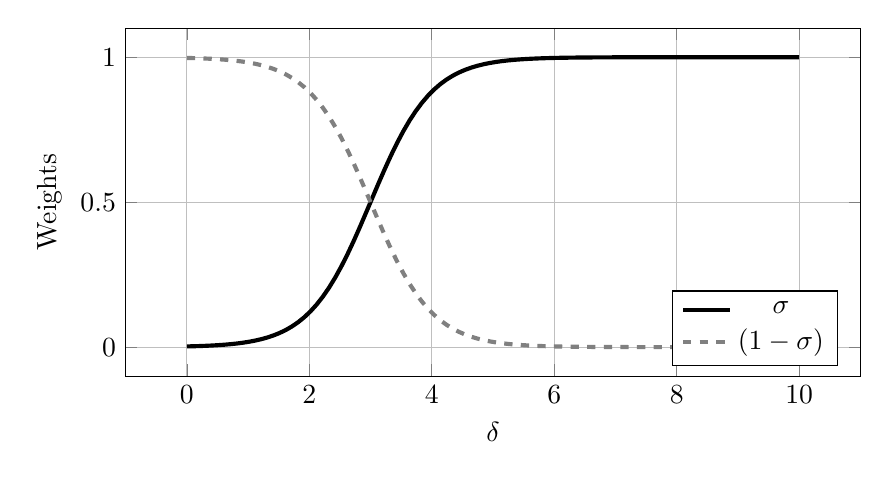
\begin{tikzpicture}%[trim axis left]
		\begin{axis}[
		  width = 0.9\textwidth,
		  height = 6cm,
		  domain = 0.001:10,
		  samples = 100,
		  grid = both,
		  xlabel = $\delta$,
		  ylabel = Weights,
		  legend pos = south east] % customize the axis environment with whatever you want (xmax,ymin,...)	  
		\addplot [color=black, solid, line width=1.5pt] {0.5*tanh(x-3)+0.5}; \addlegendentry{$\sigma$};
		\addplot [color=gray, dashed, line width=1.5pt] {1-(0.5*tanh(x-3)+0.5)}; \addlegendentry{$(1-\sigma)$};
		\end{axis}
	\end{tikzpicture}
	\caption{Plot mit Tikz (ohne Umweg über Matlab)}
\end{figure}


\begin{figure}[htb]
	% Define block styles
	\tikzstyle{decision} = [diamond, draw, %fill=green!20, 
		text width=4.0em, text badly centered, node distance=2cm, inner sep=0pt]
	\tikzstyle{block} = [rectangle, draw, %fill=green!20, 
	text width=5em, text centered, rounded corners, minimum height=2em]
	\tikzstyle{line} = [draw, -latex']
	\tikzstyle{cloud} = [draw, ellipse, %fill=orange!40,
				 node distance=3cm, minimum height=2em]
	
	\begin{center}
		\begin{tikzpicture}[node distance = 1.4cm, auto, every node/.style={font=\sffamily\scriptsize}]
		% Place nodes
		\node [block] (init) {initialize model};
		\node [cloud, left of=init] (expert) {expert};
		\node [cloud, right of=init] (system) {system};
		\node [block, below of=init] (identify) {identify candidate models};
		\node [block, below of=identify] (evaluate) {evaluate candidate models};
		\node [block, left of=evaluate, node distance=3cm] (update) {update model};
		\node [decision, below of=evaluate] (decide) {is best candidate better?};
		\node [block, below of=decide, node distance=1.9cm] (stop) {stop};
		% Draw edges
		\path [line] (init) -- (identify);
		\path [line] (identify) -- (evaluate);
		\path [line] (evaluate) -- (decide);
		\path [line] (decide) -| node [near start] {yes} (update);
		\path [line] (update) |- (identify);
		\path [line] (decide) -- node {no}(stop);
		\path [line,dashed] (expert) -- (init);
		\path [line,dashed] (system) -- (init);
		\path [line,dashed] (system) |- (evaluate);
		\end{tikzpicture}
	\end{center}
	\caption{Ablaufdiagramm mit Tikz}
\end{figure}
